
\subsection{Tipos de galaxias}

\begin{tikzpicture}[]
    % node definitions
    \node (s1) at (0, 0) {};
    \node (s2) at (1, 0) {};
    \node (s3) at (2, 0) {};
    \node (s4) at (3, 0) {};
    \node (s5) at (4, 0) {};
    % sketch
    \draw [test={1pt}{c1}{c2}, thick] (s1.center) to (s2.center);
    \draw [test={1pt}{c2}{c3}, thick] (s2.center) to (s3.center);
    \draw [test={1pt}{c3}{c4}, thick] (s3.center) to (s4.center);
    \draw [test={1pt}{c4}{c5}, thick] (s4.center) to (s5.center);
\end{tikzpicture}

\citet{peebles2021extended}

\citet{bag2021shape}

Las galaxias son los bloques de construcci\'on b\'asicos del Universo cuando se mira a las escalas m\'as grandes.
Estrictamente hablando, fueron observadas por primera vez por Sir Frederick William Herschel (1738-1822),
quien identific\'o una gran colección de objetos "nebulosos" en el cielo nocturno. Fue a partir de observaciones de Edwin Hubble (1889-1953) en la d\'ecada de 1920, que se estableci\'o claramente que esos
objetos se encontraban mucho m\'as all\'a de la V\'ia L\'actea (Hubble 1925). \\

Desde las primeras observaciones, pronto qued\'o claro que las galaxias tienen diferentes formas (morfolog\'ias)
y diferentes propiedades f\'isicas, situación que hoy en d\'ia se conoce como el \Textit{Zool\'ogico gal\'actico}. Esta diversidad hizo necesaria una "taxonomía de galaxias". La famosa \Textit{secuancia de Hubble} fue el primer esquema de clasificaci\'on morfol\'ogica consistente de galaxias, reuniendolas en 4 categor\'ias principales: el\'ipticas, lenticulares, espirales e irregulares. \\ 

\begin{itemize}
\item Las galaxias el\'ipticas (E) se caracterizan por tener isofotas casi elípticas
(contornos de brillo superficial constante). Se clasifican adem\'as como $En$ de acuerdo con
su elipticidad, donde $n$ es el entero m\'as cercano a $10(1 -b/a)$, donde $a$ y $b$ son las longitudes de su eje semimayor y semimenor, respectivamente. Emp\'iricamente, $n$
var\'ia entre 1 y 7. 
\item Las galaxias espirales (S) tienen presencia de brazos espirales alrededor
una estructura de disco delgado y una protuberancia central. Se subdividen en espirales normales y
espirales barradas (SB), seg\'un haya o no una estructura en forma de barra en
la parte central de la galaxia. A cada una de estas clases de espirales se le asignan adem\'as las letras
$a$, $b$ o $c$, seg\'un el brillo de la protuberancia en relaci\'on con el disco, lo compacto de
los brazos espirales alrededor de la galaxia y el grado en que es posible resolver las estrellas,
regiones HII y polvo en los brazos espirales. 
\item Las galaxias lenticulares (S0) son intermedias entre galaxias el\'ipticas y espirales, tienen una estructura similar a un disco, dominada por una protuberancia pero sin presencia de brazos espirales. En algunos casos, las galaxias lenticulares pueden tener una barra central, en cuyo caso se clasifican como SB0. 
\item las galaxias irregulares (Irr) son galaxias casi sin estructura perceptible (Irr I) o sin estructura (Irr II).
\end{itemize}

\begin{figure}[!h]
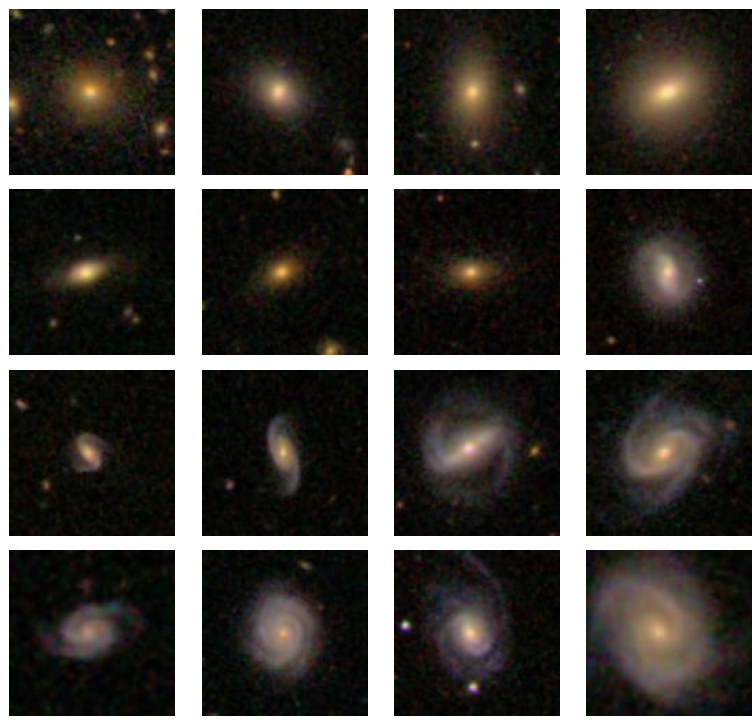
\includegraphics[width=\textwidth]{images/sdss-galaxies.png}
\caption{SDSS cutout images galaxies of diffeerent morphological type. From top to
bottom: Elliptical, Lenticular, Barred and Spiral galaxies. Each image is $48\times48\, \mbox{arcsec}^2 $}
\end{figure}


Incluso cuando la clasificaci\'on descrita anteriormente se bas\'o únicamente en la apariencia visual
de galaxias, hoy en d\'ia est\'a bien establecido que tal distinci\'on morfol\'ogica esta conectada a diferentes procesos f\'isicos y evolutivos subyacentes. Especialmente evidente de los estudios extragal\'acticos llevados a cabo a finales de los años 20 y principios de los 30 era el hecho que la distribuci\'on de las galaxias en el cielo no es uniforme sino que tienden a agruparse. \\


\begin{figure}[!h]
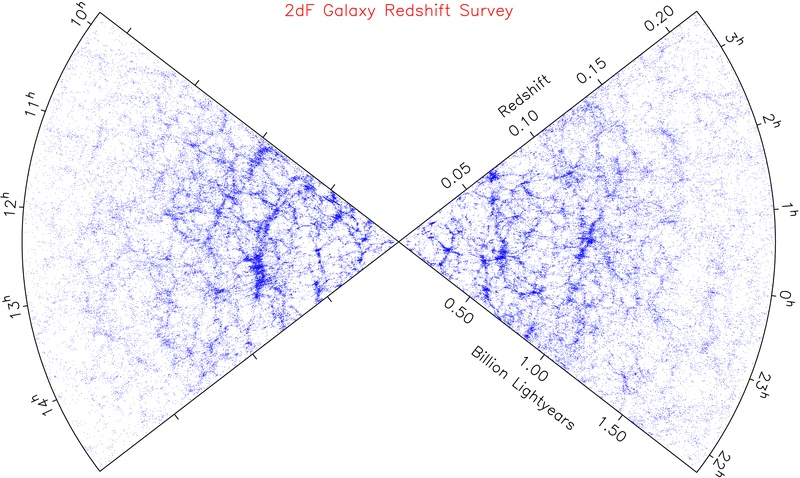
\includegraphics[width=\textwidth]{images/2dFzcone.jpg}
\caption{Galaxy distribution from the complete \href{http://magnum.anu.edu.au/~TDFgg}{2dFGRS}}
\end{figure}


Diferentes estudios en la d\'ecada de los años 80 comenzaron a encontrar fuertes correlaciones entre el tipo morfol\'ogico de las galaxias y sus ambientes. \\

El estudio de la distribuci\'on de las galaxias a gran escala y la dependencia de sus
propiedades en relaci\'on a su medio ambiente es uno de los principales objetivos de la cosmolog\'ia observacional. A partir de esta informaci\'on es posible establecer restricciones en los modelos cosmol\'ogicos. Esta es la raz\'on por la que cada vez se requieren estudios de galaxias más grandes y profundos. \\


As no single dark energy candidate or no particular modification of the theory of gravity is universally accepted as the right model to account for the alleged accelerated expansion of the universe, there is a recent trend of reconstructing the models for the observed universe through kinematical quantities \citep{DUARY2022101726}